%                                                                 aa.dem
% AA vers. 8.2, LaTeX class for Astronomy & Astrophysics
% demonstration file
%                                                       (c) EDP Sciences
%-----------------------------------------------------------------------
%
%\documentclass[referee]{aa} % for a referee version
%\documentclass[onecolumn]{aa} % for a paper on 1 column  
%\documentclass[longauth]{aa} % for the long lists of affiliations 
%\documentclass[rnote]{aa} % for the research notes
%\documentclass[letter]{aa} % for the letters 
%\documentclass[bibyear]{aa} % if the references are not structured 
% according to the author-year natbib style

%
\documentclass[letter]{aa}  

%
\usepackage{graphicx}
%%%%%%%%%%%%%%%%%%%%%%%%%%%%%%%%%%%%%%%%
\usepackage{txfonts}
%%%%%%%%%%%%%%%%%%%%%%%%%%%%%%%%%%%%%%%%
\usepackage{tabularx}
\usepackage{amsfonts}
\usepackage{bbold}
\usepackage{color}
\usepackage{transparent}
\usepackage{hyperref}
\usepackage{transparent}
\usepackage{rotating}
\usepackage{caption}
\usepackage{subcaption}

% Only include extra packages if you really need them. Common packages are:
\usepackage{graphicx}	% Including figure files
\usepackage{amsmath}	% Advanced maths commands
\usepackage{amssymb}	% Extra maths symbols
\usepackage{tablefootnote}
\usepackage[flushleft]{threeparttable}
\usepackage{dblfloatfix} 

\usepackage{natbib}
\bibpunct{(}{)}{;}{a}{}{,} 

\newcommand{\sgx}{SgXB\xspace}
\newcommand{\ulx}{ULX\xspace}
\newcommand{\sfxt}{SFXT}
\newcommand{\sg}{Sg\xspace}
\newcommand{\co}{CO\xspace}
\newcommand*{\hmxb}{HMXB\@\xspace}
\newcommand*{\lmxb}{LMXB\@\xspace}
\newcommand*{\rlof}{RLOF\@\xspace}
\newcommand*{\ns}{NS\@\xspace}
\newcommand*{\bh}{BH\@\xspace}
\newcommand*{\eg}{e.g.\@\xspace}
\newcommand*{\ie}{i.e.\@\xspace}
\newcommand*{\aka}{a.k.a. \@\xspace}
\newcommand*\diff{\mathop{}\!\mathrm{d}}
\newcommand{\mystar}{{\fontfamily{lmr}\selectfont$\star$}}
\newcommand*{\msun}{$M_{\odot}$\@\xspace}
\newcommand*{\mdotstar}{$\dot{M}_{\text{\mystar}}$\@\xspace}
\newcommand*{\mdotacc}{$\dot{M}_{\text{acc}}$\@\xspace}
\newcommand*{\ledd}{$L_{\text{Edd}}$\@\xspace}

 
%\usepackage[options]{hyperref}
% To add links in your PDF file, use the package "hyperref"
% with options according to your LaTeX or PDFLaTeX drivers.
%
\begin{document} 

%   \title{Mass transfer via wind-Roche lobe overflow in High Mass X-ray binaries}
   \title{Wind Roche lobe overflow in high mass X-ray binaries}

   \subtitle{A possible mass transfer mechanism for Ultraluminous X-ray sources}

   \author{I. El Mellah
          \inst{1}
          \and
          J. O. Sundqvist
          \inst{2}
          \and
          R. Keppens
          \inst{1}
          }

   \institute{Centre for mathematical Plasma Astrophysics, 
   			 Department of Mathematics, KU Leuven, 
   			 Celestijnenlaan 200B, B-3001 Leuven, Belgium\\
              \email{ileyk.elmellah@kuleuven.be}
         \and
             KU Leuven, Instituut voor Sterrenkunde, 
             Celestijnenlaan 200D, B-3001 Leuven, Belgium
             }

   \date{Received ...; accepted ...}

% \abstract{}{}{}{}{} 
% 5 {} token are mandatory
 
  \abstract{Ultra-luminous X-ray sources (\ulx) have such high X-ray luminosities that they were long thought to be accreting intermediate mass black holes. Yet, some have been shown to display periodic modulations and coherent pulsations, suggestive of a neutron star in orbit around a companion and accreting at super-Eddington rates. The question of the mass transfer mechanism suitable to feed the accretor at such high rates remains open. In this letter, we propose that Supergiant X-ray binaries (\sgx) could undergo a \ulx phase when the wind from the donor star is highly beamed towards the compact accretor. Since the star does not fill its Roche lobe and that a significant fraction of the stellar wind still escapes the system, this mass transfer mechanism known as "wind - Roche lobe overflow" can remain stable even for large mass ratios. Based on realistic acceleration profiles derived from spectral observations and modeling of the stellar wind, we perform three-dimensional ballistic simulations to evaluate the fraction of the wind captured by the compact object. We identify the orbital and stellar conditions for a \sgx to be the stage of mass transfer rates matching the expectations for \ulx and show that the transition from \sgx to \ulx luminosity levels is progressive. These results prove that high stellar Roche lobe filling factors are not necessary to funnel large quantities of material into the Roche lobe of the accretor. Slow and dense winds such as the ones emitted by the Wolf-Rayet star in M101 ULX-1 or the late B9 Supergiant in P13 ULX-1 are enough to lead to a highly beamed wind and a significantly enhanced mass transfer rate.}

   \keywords{XXX accretion, accretion discs -- X-rays: binaries -- stars: neutron, black holes, supergiants, winds -- methods: numerical}

   \maketitle
%
%________________________________________________________________

\section{Introduction}

Ultra-luminous X-ray sources are spatially-unresolved persistent sources with luminosities in excess of 10$^{39}$erg$\cdot$s$^{-1}$ \citep[see][for a recent review]{Kaaret2017}. This X-ray luminosity threshold corresponds approximately to the Eddington luminosity \ledd of a 10\msun black hole (\bh), the limit above which isotropic accretion onto a body of this mass is thought to be self-regulated by the radiative field it produces \citep{Rappaport2005}. They are found off-nuclear in galaxies within a couple of 10Mpc, ruling against a supermassive \bh origin. If the emission is not beamed, such accretion rates can only be sustained for accretors of at least several 10 to several 100\msun bodies, suggestive of the long awaited population of intermediate mass \bh \citep{Colbert1999}. The accretor in the ULX M82 X-1 \citep{Brightman2016} has been showed to be 20 to 35\msun \bh while the observation of gravitational waves emitted by merging compact objects unearthed \bh of several 10\msun \citep{Abbott2016}.

However, the detections of coherent pulsations and cyclotron resonance scattering features from several ULX demonstrate that other ULX host super-Eddington accreting neutron stars \citep[\ns,][]{Bachetti2014,Furst2016,Israel2017,Carpano2018,Brightman2018}. In one of them, NGC7793 P13 (hereafter P13), \cite{Motch2014} identified a stellar spectrum consistent with a 20\msun B9Ia star, in a $\sim$64 days orbit with an X-ray source they assumed to be a \bh but which later turned out to be an accreting \ns \citep{Furst2016}. It was further argued that the star has to fill its Roche lobe because the stellar mass loss rate would be too low and wind accretion would not be able to lead to a significant fraction of the stellar wind being captured by the accretor. On the other hand, \cite{Liu2013} showed that in M101 ULX-1 (hereafter M101), the Helium emission lines are best explained by a Wolf-Rayet donor star twice smaller than its Roche lobe. It suggests that mass transfer rates suitable for \ulx X-ray luminosity levels are possible without Roche lobe overflow (\rlof). Finally, in two ULX, near-infrared counterparts consistent with red supergiant donors have been identified \citep{Heida2015,Heida2016}.
%rules out a mass transfer towards the accreting stellar mass \bh via Roche lobe overflow (\rlof), and brings up the question of the capacity of wind mass transfer to actually lead to large mass accretion rates.
%However, such a large mass ratio (defined as the mass of the donor divided by the mass of the accretor) would most certainly lead to unstable \rlof, even in the most stabilizing configurations \citep{Pavlovskii2017}.

Most ULX hosting a stellar mass accretor are now thought to be the high mass accretion rate end of the Supergiant X-ray binaries (\sgx), where the wind from a supergiant donor star acts as a reservoir of matter tapped by the orbiting compact object. The X-ray luminosity functions of \sgx and \ulx follow the same power-law, without apparent break \citep{Gilfanov2004,Swartz2011}. Super-orbital periods are observed in \sgx \citep{Corbet2013} and in \ulx \citep{Walton2016,Fuerst2018}. The main spectral differences between \sgx and \ulx can be attributed either to the nature of the donor or to different accretion geometry in the immediate vicinity of the accretor \citep{Kaaret2017}. All these elements support the idea that both types of objects belong to the same population and that the mass transfer mechanism at the orbital scale might be qualitatively the same.

The final absolute X-ray luminosity $L_X$ released by accretion onto a compact object fed by a stellar companion depends on :
\begin{itemize}
\item \mdotstar the stellar mass loss rate.
\item $\dot{M}$ the rate at which mass is transferred from the star into the domain of gravitational influence of the accretor.
\item \mdotacc the mass which actually ends up being accreted onto the compact object.
\item $\zeta$ the efficiency of the conversion of accreted mass to radiation, set here to 10$\%$.
\end{itemize} 
with \mdotstar $>\dot{M}>$ \mdotacc. In this letter, we set aside the question of how super-Eddington accretion itself proceeds in the vicinity of the accretor \ie how the compact object can accrete at a rate \mdotacc leading to $L_X=\zeta$\mdotacc$c^2>$\ledd. Rather, we ask whether stellar material can be transferred to the compact object at a rate $\dot{M}$ high enough to reach the ULX luminosity level, without necessarily assuming \rlof. In the context of symbiotic binaries, \cite{Mohamed2007} showed that a wind speed low enough compared to the orbital speed could lead to a significant enhancement of the mass transfer rate. This mechanism, known as wind Roche lobe overflow (wind-\rlof), is characterized by a strongly beamed wind in the orbital plane and towards the accretor. This mass transfer does not undergo runaway \rlof expected for high mass ratios\footnote{Defined as the mass of the donor divided by the mass of the accretor.} since the process is not conservative and the star does not fill its Roche lobe, although a fraction of the stellar wind large enough to reach the \ulx level might still be captured by the accretor.  

% ------------------------------------------------
\section{Stellar winds in SgXB}
\label{sec:}
% ------------------------------------------------

%\begin{figure}
%\begin{subfigure}{.5\textwidth}
%\centering
%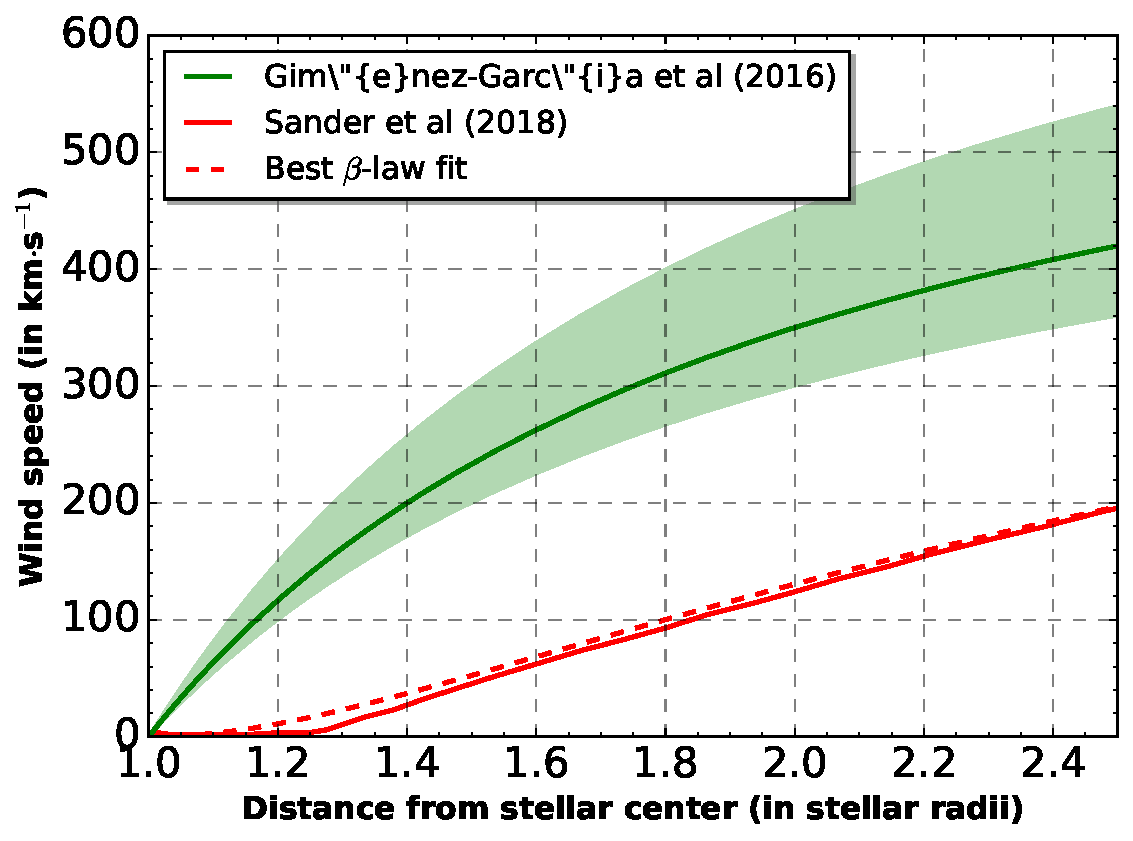
\includegraphics[width=0.99\columnwidth]{Pictures/vel_prof.pdf}
%  \label{fig:vel_prof}
%\end{subfigure}
%\phantom{p}\\
%\begin{subfigure}{.5\textwidth}
%\centering
%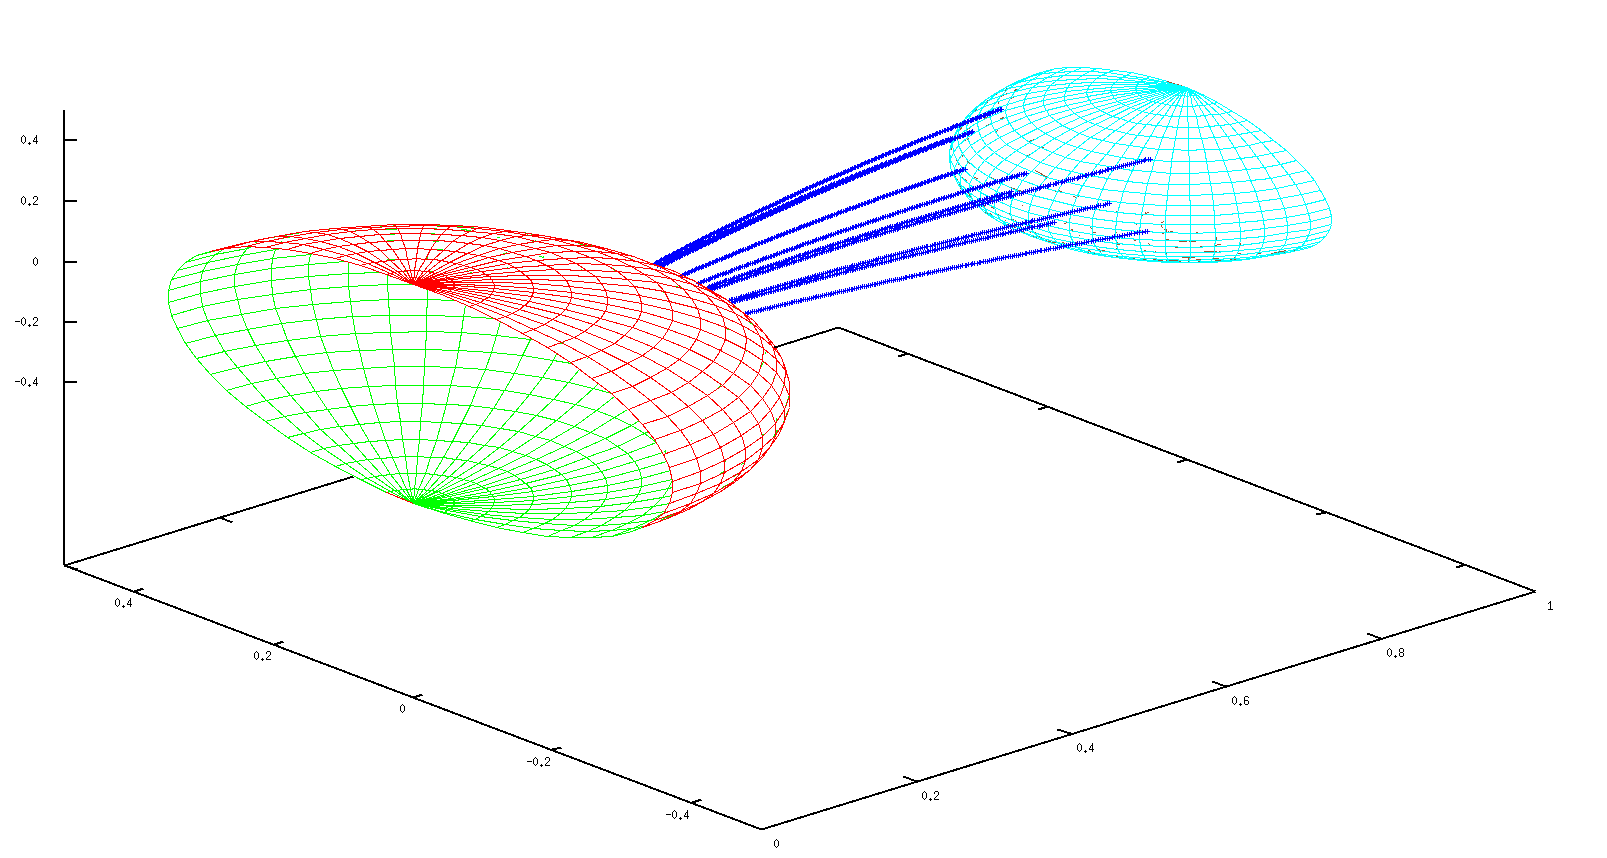
\includegraphics[width=0.99\columnwidth]{Pictures/3D.png}
%  \label{fig:3D}
%\end{subfigure}
%\caption{(upper panel) Wind velocity profiles of a representative B0.5 Ib supergiant star, HD 77581 \citep[the donor star in Vela X-1, where the accreting \ns lies at $\sim$1.8 stellar radii][]{Hiltner1972,Forman1973}. The green solid line is the $\beta$-velocity profile deduced by \cite{Gimenez-Garcia2016} from observations, while the green shaded region shows the uncertainties on the terminal wind speed. \cite{Sander2017} computed the hydrodynamic atmosphere solution for the wind stratification (red solid line), here fitted by a $\beta$-velocity profile (dashed red line). (lower panel) Illustration of the integration of the streamlines (orange) from the stellar surface (blue) to the Roche lobe of the accretor (transparent green).}
%\label{fig:setup}
%\end{figure} 

We solve the ballistic equation of motion in the three-dimensional co-rotating frame of a binary system, for test-masses starting at the stellar surface and subjected to the two gravitational forces, the non-inertial forces and the wind acceleration. We use the numerical integrator described in \cite{ElMellah2016a}. In \sgx hosting an O/B Supergiant, the wind launching mechanism relies on the resonant absorption of UV photons by partially ionized metal ions \citep{Lucy1970,Castor1975}. In an isotropic situation, it can be shown to produce radial velocity profiles which obey the $\beta$-law :
\begin{equation}
\varv_{\beta}(r)=\varv_{\infty}\left(1-R_{\text{\mystar}}/r\right)^{\beta}
\end{equation}
with $R_{\text{\mystar}}$ the stellar radius, $\varv_{\infty}$ the terminal wind speed and $\beta$ which represents the efficiency of the acceleration \ie how fast the wind reaches its terminal speed : the lower $\beta$, the earlier $\varv_{\infty}$ is matched. Notice that, although the wind launching mechanism of cool stars is still largely unknown, the wind velocity profiles observed around red supergiant and asymptotic giant branch stars turn out to be in reasonable agreement with this law beyond the condensation radius \citep{Decin2006,Decin2010}. The terminal wind speeds are much lower than for winds from hot stars but they display similar $\beta$ exponents and mass loss rates above 10$^{-5}$\msun$\cdot$yr$^{-1}$ are common \citep{DeBeck2010}. In Figure\,\ref{fig:vel_prof}, we plotted the wind velocity profile of the hot supergiant HD 77581 (the donor star in the classic \sgx Vela X-1). From observations of UV spectral lines, \cite{Gimenez-Garcia2016} derived the best $\beta$-law in solid green ($\varv_{\infty}\sim 700$km$\cdot$s$^{-1}$, $\beta=1$) while \cite{Sander2017} computed the hydrodynamic atmosphere solution for the wind stratification, best-fitted by a $\beta$-law with $\varv_{\infty}\sim 500$km$\cdot$s$^{-1}$ and $\beta\sim 2.3$ (red dashed curve). Given these uncertainties, we evaluate the wind acceleration in an empirical manner by relying on representative velocity profiles from which we can derive steady radial line-driven accelerations. We also need to assume that the departure from the isotropic case due to the presence of an orbiting accretor does not significantly alter the radial component of the wind acceleration, still given by $v_{\beta}\diff_rv_{\beta}$. 
%Close from the star, where the line-driven acceleration peaks, non isotropic effects on the mass loss rate are neglected.

To evaluate the fraction of wind captured $\mu=\dot{M}/$\mdotstar, we need to define the region of gravitational influence of the accretor. It is given by its Roche lobe if the accretion radius $R_{acc}$ is larger than the Roche lobe radius, and the sphere of radius $R_{acc}$ centered on the accretor otherwise. $R_{acc}$ has been shown in \cite{ElMellah2015} to be an accurate order of magnitude of the effective cross section of a point mass accreting from a planar uniform wind for Mach numbers of the incoming flow above 4, a condition quickly matched in \sgx. It reads :
\begin{equation}
R_{acc}=2GM_{\bullet}/v_{\beta}(r=a)
\end{equation}
with $a$ the orbital separation, $G$ the constant of gravity and $M_{\bullet}$ the mass of the accretor. In \sgx, the accreting compact object lies deep in the wind, in a region where the wind is still accelerating. Given the uncertainties which remain on this regime and the important dependency of the accretion radius on the wind speed, we need to consider a variety of $\beta$ exponents : for instance, the two wind velocity profiles derived for HD 77581 in Figure\,\ref{fig:vel_prof} lead to a discrepancy of $\sim$10 on the accretion radius of the \ns, lying at $a\sim1.8R_{\text{\mystar}}$ from the stellar center.

In dimensionless form, the solutions of the equation of motion depend only on the mass ratio $q$, the filling factor\footnote{Ratio of the stellar radius by the Roche lobe radius \citep{Eggleton1983}.} $f$, the $\beta$ exponent and the ratio of the terminal wind speed by the orbital speed $\eta=\varv_{\infty}/\varv_{orb}$, with $\varv_{orb}=2\pi a/P_{\text{orb}}$ and $P_{\text{orb}}$ the orbital period. In particular, these 4 parameters entirely determine the ratio $\mu$ of stellar wind significantly beamed towards the accretor. We quantify it by monitoring the fraction of integrated streamlines entering the domain of gravitational influence of the accretor.

\begin{figure}
\centering
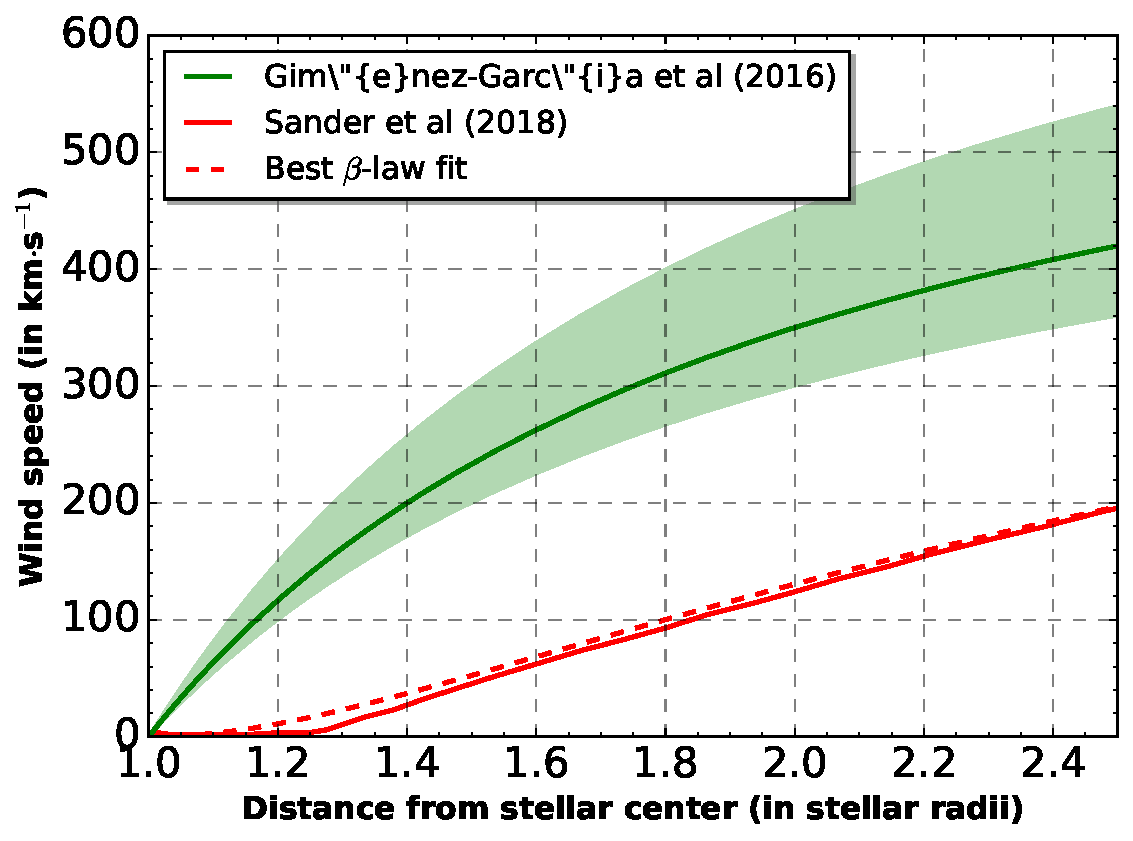
\includegraphics[width=1\columnwidth]{Pictures/vel_prof.pdf}
\caption{Wind velocity profiles of the B0.5 Ib supergiant, HD 77581. The green solid line is the $\beta$-velocity profile deduced by \cite{Gimenez-Garcia2016} (the green shaded region shows the uncertainties on the terminal wind speed) while \cite{Sander2017} derived a sensibly smoother profile (red lines).}
\label{fig:vel_prof}
\end{figure} 
%% - - - - - - - - - - - - - - - - - - - - - - - - 
%\subsection{Empirical proxy to deduce acceleration from beta-laws}
%\label{sec:}
%% - - - - - - - - - - - - - - - - - - - - - - - - 
%
%First of all, we 
%
%
%% - - - - - - - - - - - - - - - - - - - - - - - - 
%\subsection{The equation of motion}
%\label{sec:}
%% - - - - - - - - - - - - - - - - - - - - - - - - 

\begin{figure*}[!b]
\centering
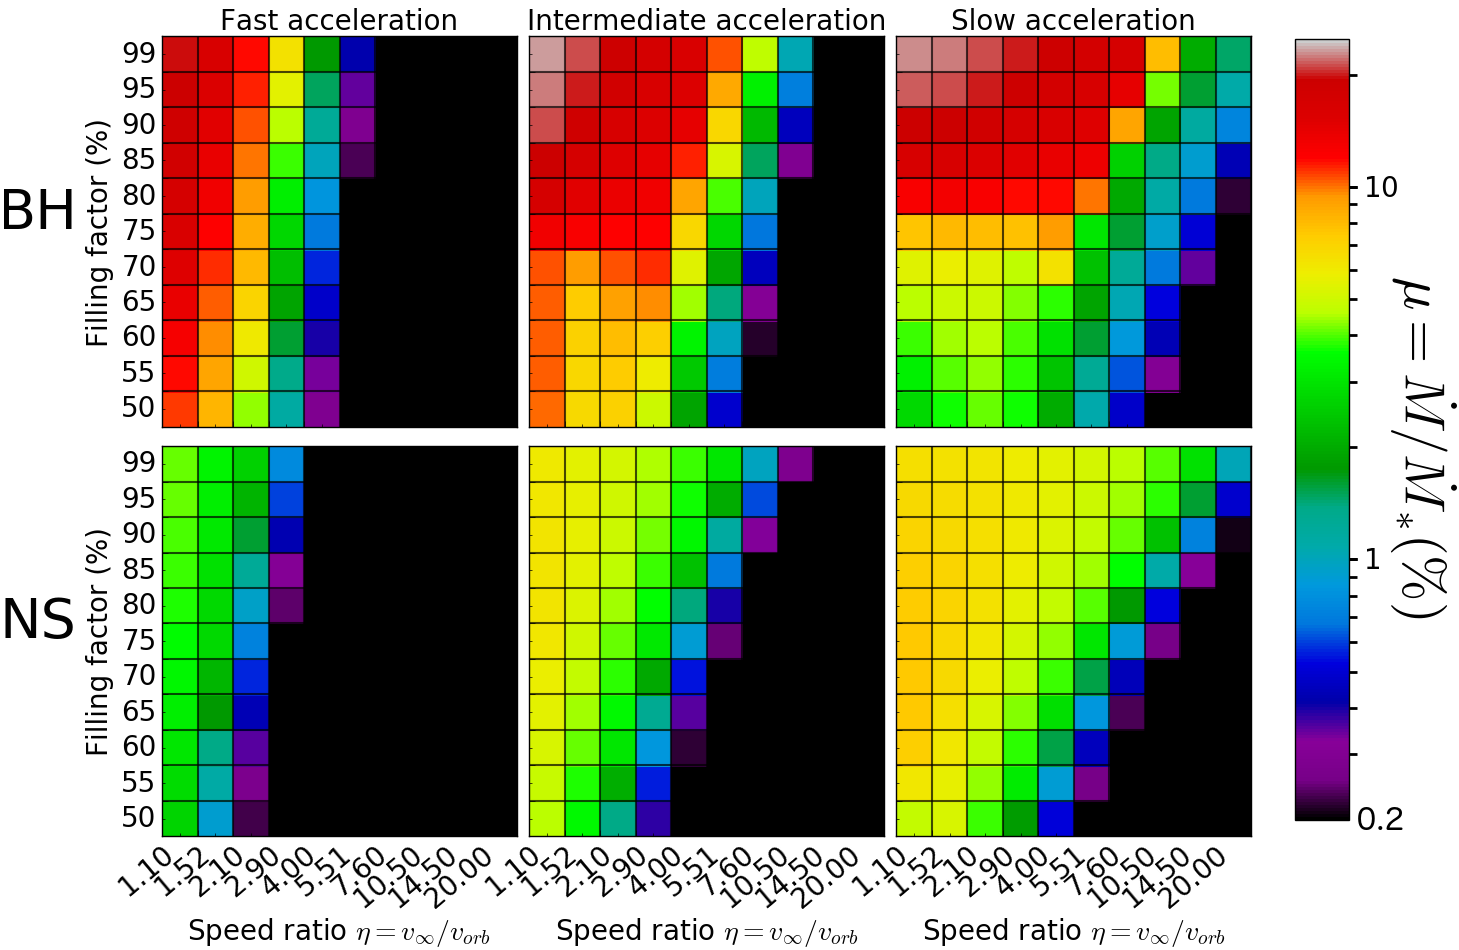
\includegraphics[width=2\columnwidth]{Pictures/mdot_grid.png}
\caption{Logarithmic color maps of the fraction $\mu$ of stellar wind captured by the accretor as a function of the stellar filling factor and of the ratio of the terminal wind speed by the orbital speed. From left to right, $\beta=$1, 2 and 3. The first (resp. second) row stands for a mass ratio of 2 (resp. 15).}
\label{fig:mdot}
\end{figure*} 

% ------------------------------------------------
\section{Mass transfer via wind-RLOF}
\label{sec:}
% ------------------------------------------------

% - - - - - - - - - - - - - - - - - - - - - - - - 
\subsection{Fraction of stellar wind available for accretion}
\label{sec:}
% - - - - - - - - - - - - - - - - - - - - - - - - 

We probe a range of parameters realistic for \ulx, whether the donor star is a Wolf-Rayet or a supergiant. The few orbital periods and mass measures available indicate that the orbital speed might vary by a factor of a few from a \ulx to another, while the terminal wind speeds of cool supergiants is generally more than an order of magnitude lower than for hot supergiants : we span values of $\eta$ from 1.1 to 20. We work with a $\beta$ exponent of 1, 2 and 3, which means a more progressive acceleration up to the terminal speed. Observed filling factors lie between 50\% and 100\% (\rlof). Two extreme mass ratios have been considered, $q=$2 and $q=$15, which correspond respectively to a stellar mass \bh and a \ns accreting from a $\sim$20\msun supergiant.

Figure\,\ref{fig:mdot} illustrates the evolution of the fraction of wind captured with the 4 dimensionless parameters of the problem. The main parameter is $\eta$ : when the terminal wind speed gets a few times larger than the orbital speed, the effective cross-section set by the accretion radius decreases quickly and much below the radius of the Roche lobe of the accretor. This effect is tempered for slowly accelerating winds (\ie for high $\beta$) which, provided the distance from the photosphere to the accretor is small (\ie for large $f$), are still far from their terminal wind speed when they enter the Roche lobe of the accretor. On the revert, the dependency of $\mu$ on the filling factor vanishes when the wind accelerates quickly because then, by the time it reaches the accretor, the wind has almost reached its terminal speed. Smooth and slow wind launching leads to a significant contribution of the high latitude stellar regions : the flow is strongly beamed in the orbital plane and the value of $\mu$ surges. 

%As a rule of thumb AND IN ORDER OF IMPORTANCE, the dynamical range and the sensitivity of $\mu$ is the following : an increase in the ratio of the wind speed at the orbital separation by the orbital speed by a factor of 10 translates into a decrease of $\mu$ by 3 orders of magnitude. A filling factor varying from 50 to 99\% leads to an increase of $\mu$ by a factor $\sim$ 2 to 4 ; a mass ratio varying from 2 to 15 leads to an increase by a factor $\sim$ 

%A comparison to BHL formula (Fig.4)

% - - - - - - - - - - - - - - - - - - - - - - - - 
\subsection{Accretion luminosity}
\label{sec:}
% - - - - - - - - - - - - - - - - - - - - - - - - 

The first insight revealed by this analysis is the identification of the configurations where \ulx can not be the product of mass transfer via wind-\rlof and can be explained only if the star fills its Roche lobe. In Figure\,\ref{fig:mdot}, we represented in black the regions where $\mu$ is inferior to 0.2\%, the minimum fraction of stellar wind captured under which wind-\rlof (and a fortiori wind accretion) is not enough to reach 10$^{39}$erg$\cdot$s$^{-1}$, even for a stellar mass loss rate as high as 10$^{-4}$\msun$\cdot$yr$^{-1}$ :
\begin{equation}
\mu_{\text{min}}\sim 0.2\%\left(\frac{10\%}{\eta}\right)\left(\frac{10^{-4}\text{\msun}\cdot\text{yr}^{-1}}{\text{\mdotstar}}\right)\left(\frac{L_X}{10^{39}erg\cdot s^{-1}}\right)
\label{eq:lim}
\end{equation} 
Given the maximal $\mu$ we found at $\sim$20\%, mass transfer via wind-\rlof in a \ulx is only possible for stellar mass loss rates above 10$^{-6}$\msun$\cdot$yr$^{-1}$.

%: indeed, capturing a large fraction of the wind from the donor star is a necessary condition to reach significant mass transfer rates, but it is not a guarantee. 

%final mass accretion rate \mdotacc$<\dot{M}$ leading to the emission of X-rays is determined by the fraction of this mass being accreted, which depends on the geometry of the flow within the Roche lobe or within the accretion sphere of the compact object. 
%Hydrodynamics simulations within this region suggest that, depending on how fast the flow can radiate away the energy it gains as it is adiabatically compressed and/or shocked, the mass accretion rate can vary by a factor up to 10 \cite{ElMellah2018}. To a lesser extent, it can also be altered by the clumpiness of the wind \citep{Sundqvist2017,ElMellah}.
%X-ray ionizing feedback : However, at these X-ray luminosities, even with an orbital period as long as in P13, we do expect a significant X-ray ionizing feedback on the wind and a serious departure from the classic wind launching mechanism \citep{Hatchett1977,Stevens1991}. \cite{Ho1987} already pinpointed that a high luminosity solution could exist when the wind was highly ionized. For Vela X-1, their low luminosity solution matches the few 10$^{36}$erg$\cdot$s$^{-1}$ observed but once the wind is in the high ionization stage, they find an X-ray luminosity 2,000 times larger, matching a \ulx level, although such a flare has never been observed in Vela X-1.
%The final mass accretion rate depends on the compressibility of the accreted flow \citep{MacLeod2017}, on the clumpiness of the wind being captured \citep{Sundqvist2017}, on the X-ray ionizing feedback \cite{Manousakis2015c} and on the outflows expected in the case of super-Eddington accretion \citep{Pinto2016a}.

Rather than covering the large scope of regimes possible, let us focus on 3 donor stars in one \sgx and two \ulx. In the \sgx Vela X-1, \cite{Gimenez-Garcia2016} reported a stellar mass loss rate $M_{\text{\mystar}}\sim6.3$\msun$\cdot$yr$^{-1}$ for the B0.5 Ib supergiant donor star. In M101, \cite{Liu2013} computed a mass loss rate of 2$\cot$10$^{-5}$\msun$\cdot$yr$^{-1}$ for the Wolf-Rayet donor. In P13, the stellar mass loss rate of the B9 Ia supergiant donor star might well have been underestimated : in \cite{Motch2014}, it is assumed that the donor star fills its Roche lobe on the basis that the wind mass loss rate derived by \cite{Kudritzki1999} would be inferior to 10$^{-6}$erg$\cdot$s$^{-1}$. However, \cite{Kudritzki1999} did not include late type B supergiants in their study because of the difficulty to measure their terminal wind speed \citep{Howarth1997}. \cite{Vink2000a} and \cite{Vink2001} provided fits for the mass loss rate and the terminal wind speed which extend below the second bi-stability jump \citep[\ie for effective temperatures $T_{eff}\lesssim12kK$][]{Lamers2000} : with the values reported by \cite{Motch2014} ($T_{eff}\sim$11kK, stellar luminosity L$_{\text{\mystar}}\sim10^{5.1}L_{\odot}$ and stellar mass $\sim$20\msun), the mass loss rate is $\sim$10$^{-5}$\msun$\cdot$yr$^{-1}$ for solar metallicity (A. A. C. Sanders, private communication), comparable to the one found M101.

Let us now estimate the 4 dimensionless parameters for each system. For P13, \cite{Fuerst2018} determined orbital elements which indicate, in combination with the stellar parameters above, $f>90\%$, $q\sim 15$ and $\varv_{orb}=$100 to 200km$\cdot$s$^{-1}$ (for an inclination angle of respectively the maximum one set by the absence of eclipse, $\sim$55$^{\circ}$, and 20$^{\circ}$). At the bi-stability jump, the terminal wind speed should be between 0.7 and 1.3 times the escape velocity at the stellar surface \ie $\varv_{\infty}=$150 to 300km$\cdot$s$^{-1}$, hence $\eta=1$ to 3. According to Figure\,\ref{fig:mdot}, $\mu_{\text{min}}=6\%$ for the observed $L_X\sim 3\cdot 10^{39}$erg$\cdot$s$^{-1}$ is reached either for $\eta\le2$ or $\eta=3$ and $\beta>1$. Stellar material at a sufficiently high rate could then be supplied via wind-\rlof. 

In M101, the mass function indicates that the accretor must be a \bh, with $q\sim$2 for an intermediate orbital inclination \citep{Liu2013}. Their best fit to explain the Helium emission lines leads to a filling factor of at most $f=50\%$ and a terminal wind speed of 1,300km$\cdot$s$^{-1}$, 3 to 4 times larger than the orbital speed. It leads to $\mu=$3 to 10\%, in agreement with the mass accretion rate required to produce a \ulx. Since the star does not fill its Roche lobe at all, this \ulx can only be explained with the wind-\rlof mass transfer mechanism.
%Notice that if the accretor turns out to be a \ns, since the fraction of stellar wind captured via wind-\rlof would be too low and the star does not fill its Roche lobe, no known mass transfer mechanism could explain the origin of this \ulx.

Vela X-1 has dimensionless parameters which lie in the same ranges as P13, but is crippled by its stellar mass loss rate, 20 times lower and possible effects which prevents a significant fraction of the mass captured from eventually being accreted. Hydrodynamics simulations within the Roche lobe of the compact object suggest that, when the flow can not radiate away the energy it gains as it is adiabatically compressed and/or shocked, the mass accretion rate \mdotacc can be lowered by a factor $\sim$10 compared to the mass captured rate \citep{ElMellah2018}. Since the wind speeds are comparable in \ulx and \sgx, the flow density in Vela X-1 must be much lower than in P13 or M101, leading to a less efficient radiative cooling. Also, the very high X-ray luminosities in \ulx are expected to considerably ionize the wind and inhibit its acceleration \citep{Blondin1991,Manousakis2015c}, even for orbital separations as large as in P13, which participates in the efficient accretion of the material captured in \ulx. \cite{Ho1987} already pinpointed that a high luminosity solution could exist when the wind was highly ionized. For Vela X-1, the low luminosity solution matches the few 10$^{36}$erg$\cdot$s$^{-1}$ observed but once the wind is in the high ionization stage, the X-ray luminosity is 2,000 times larger, matching a \ulx level, although such a flare has never been observed in Vela X-1. To a lesser extent, the fraction of mass captured ending up being accreted can also be altered by the clumpiness of the wind \citep{Sundqvist2017,ElMellah}. These combined effects might explain why many \sgx have luminosities lower than the Eddington luminosity of a \ns or a stellar mass \bh.

%\begin{center}
%\begin{table}[!b]
%\caption{Scaled X-ray luminosity of a classic \sgx (Vela X-1) and of a \ulx (P13) assuming the same fraction of wind captured ($\mu\sim$ 5\% for $q=15$, $f=95\%$, $\beta=2$ and $\eta=2$).}
%\label{tab:params}
%\centering
%\begin{tabularx}{0.83\columnwidth}{c|c|c}
%   & Vela X-1 & P13 \\
%  \hline
%  $\mu=\dot{M}/\dot{M}_{\text{\mystar}}$ & \multicolumn{2}{c}{$\sim$ 5\%} \\
%  \hline
%  $\dot{M}_{acc}/\dot{M}$ & 4\%  & 40\% \\
%  \mdotstar & 5$\cdot$10$^{-7}$M$_{\odot}\cdot$yr$^{-1}$ & 10$^{-5}$M$_{\odot}\cdot$yr$^{-1}$ \\
%  $L_X$ & 5$\cdot$10$^{36}$erg$\cdot$s$^{-1}$ & 5$\cdot$10$^{39}$erg$\cdot$s$^{-1}$ \\
%\end{tabularx}
%\end{table}
%\end{center}

% ------------------------------------------------
\section{Discussion and conclusions}
\label{sec:}
% ------------------------------------------------

%\begin{figure}
%\centering
%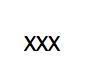
\includegraphics[width=0.99\columnwidth]{Pictures/BHL.png}
%\caption{XXX}
%\label{fig:BHL}
%\end{figure}

We showed that efficient mass transfer without \rlof could occur in a binary system from a Supergiant donor star to its compact accretor in \sgx. When the wind is slow enough compared to the orbital speed to see its dynamics significantly altered by the Roche potential, it is beamed towards the accretor. Under these conditions, we also observe a density enhancement in the orbital plane which considerably increases the fraction of the stellar wind captured and which can reach up to several 10\% : wind \rlof not only bridges the gap between \rlof and wind accretion but introduces new features. If the mass loss rate of the star is large enough, it can result in a mass available for accretion being supplied at a rate suitable to produce X-ray accretion luminosity of the order of the ones observed in \ulx. The final mass accretion rate though depends also on the compressibility of the flow, on the X-ray ionizing feedback and on the clumpiness of the wind being captured.

Some \ulx are also expected to undergo \rlof mass transfer which is bound to be unstable when the mass ratio is as high as in P13 \citep{King2002,Rappaport2005}. This mechanism is the most reliable scenario when the stellar mass loss rate is found to be smaller than 10$^{-6}$\msun$\cdot$yr$^{-1}$ or for hyperluminous X-ray sources such as ESO 243-49 HLX-1 where the X-ray luminosity can be as high as $\sim$10$^{42}$erg$\cdot$s$^{-1}$ \citep{Farrell2009,Webb2017}. Alternatively, in \ulx where the donor star has a sufficient mass loss rate and is found to not fill its Roche lobe such as M101 ULX-1 \citep{Liu2013}, wind-\rlof provides an accurate description of the geometry of the flow. Regardless from the nature of the wind-launching mechanism, the same arguments apply to the red supergiant donors identified in a couple of ULX \citep{Heida2015,Heida2016}. Due to their low terminal speeds and high mass loss rates, they are good candidates to transfer large amounts of mass via wind-\rlof \citep{Mohamed2007,DeVal-Borro2017} and to be well described by the formalism we developed, even for long orbital periods.

With this letter, we emphasize on the compelling need to improve our knowledge of the nature of the donor star and in particular of its mass loss to understand not only \sgx but also the high mass accretion tail of the distribution, \ulx. In this attempt, observational campaigns have been carried out \cite[see \eg][]{Heida2014}. Theoretical arguments have been made to constrain the donor star but they often presuppose a \rlof mass transfer and thus, might not hold for any \ulx \citep{Karino2017}. If wind-\rlof is ruled out for low stellar mass loss rates or hyperluminous X-ray sources, it is a possible alternative scenario when the wind is slow enough to lead to a significant mass transfer enhancement. 

In several \ulx, the presence of a disc has been inferred from super-orbital modulations or systematic spinning up of the \ns \citep[\eg in P13,][]{Fuerst2018}. A disc can form only if the wind is slow enough \citep{Illarionov1975} but in a pure wind accretion formalism, the mass accretion rate is given by the Bondi-Hoyle-Lyttleton formula and increases quickly when the wind speed decreases. \cite{Tutukov2016} noticed that in IC 10 X-1 and NGC 300 X-1, two systems where a stellar mass \bh accretes from a Wolf-Rayet companion, no wind speed could explain both the accretion disc and the limited X-ray luminosity of 10$^{38}$erg$\cdot$s$^{-1}$. The wind-\rlof mechanism, fully compatible with the formation of a wind captured disc while not necessarily leading to large mass accretion rates, solves this issue \citep{ElMellah2018}. 

Last, due to its enhanced efficacity while still being stable, this mass transfer mechanism could have important consequences on population synthesis of binary systems. The results presented here provide the community with estimates for the mass transfer rate as a function of a limited number of dimensionless parameters.

%For P13, NGC 5907 ULX-1 and M82 X-2, he X-ray luminosity \cite{Karino2017} . among the 3 \ns -hosting \ulx with known orbital periods recently studied by \cite{Karino2017} (P13, NGC 5907 ULX-1 and M82 X-2), only M82 X-2 fits the   

%Pure wind \rlof \ie situations where the wind speed is large compared to the orbital speed, can never lead to \ulx luminosity levels, even for large stellar mass loss rates, given the fast . 

%Similar components as the ones found in \sgx. X-ray binaries have lower luminosities though. Neither RLOF nor wind BHL can reach these levels. RLOF, ~LMXB, limited by the transverse section of the channel @ L1 while fast winds (~sgx) mean low capture cross-sections. The first is essentially limited by the small sound speed compared to the orbital speed while the second is limited by the large wind speed with respect to the orbital speed. => wind-RLOF configuration leading to enhanced accretion, best of both worlds when the stellar mass loss rate is large. \cite{King2002} suggested that above a mass ratio unity, unstable RLOF mass transfer occurs on a thermal time scale and lead to high mass accretion rate onto the compact companion. However, \cite{Pavlovskii2017} recently found that RLOF mass transfer can be stable for large q, up to 7.5. Not high enough though to match the mass ratio in P13 where the stellar mass is at least 10 times larger than the mass of the accreting \ns.

\begin{acknowledgements}
IEM is grateful to Felix F\"{u}rst, Marianne Heida, Selma De Mink, Philipp Podsiadlowski, Saul Rappaport and Timothy P. Roberts for insightful exchanges on the possible scenarios leading to ultra-luminous X-ray sources. IEM wishes to thank Andreas Sander and Jorick Vink for their estimates on the stellar mass loss rates of hot stars, and Leen Decin for her description of the stellar outflow of cool stars. IEM has received funding from the Research Foundation Flanders (FWO) and the European Union's Horizon 2020 research and innovation program under the Marie Sk\l odowska-Curie grant agreement No 665501. IEM and JOS thank the Instituto de F\'{i}sica de Cantabria for its hospitality and for sponsoring a meeting which brought together the massive stars and X-ray binaries communities.
% THANK REFERREE
\end{acknowledgements}

%-------------------------------------------------------------------

\bibliographystyle{aa} %agsm}
\begin{tiny}
\bibliography{/Users/Ileyk/Documents/Bibtex/article_ULX_no_url}
\end{tiny}

\end{document}